\documentclass{article}
\usepackage{amsmath}
\usepackage{graphicx}
\usepackage{float}

\setlength{\parindent}{0em}
\setlength{\parskip}{1em}

\title{Assignment 1}
\author{Joshua Hwang (44302650)}
\date{27 February}

\begin{document}
\maketitle

\section{Airplane failure}
$A$ is the event the plane can fly. Given $A_1$, $A_2$, $A_3$ and $A_4$ are the
chances those respective engines are working,
the set of $A$ can be represented as
\begin{align*}
    A = (A_1 \cup A_2) \cap (A_3 \cup A_4)
\end{align*}

\section{Probability of armed}
The population of King's Landing can be considered the set $K$.
Consider the sets $D$ and $S$ of people who own daggers and sword in King's
Landing respectively.

From the information provided we produce the following equations. The reader
may notice we're not giving the absolute value of the population when using the
$||$ notation. The notation was used to easily communicate proportions instead
since that is the only information we've been given.
\begin{align}
    |D \cap S| &= 10\% \label{eq:intersect} \\
    |(D \cup S)^c| &= 30\% \label{eq:complement} \\
    \frac{|(D \cap S)|}{|D|} &= 25\% \label{eq:daggers} \\
    |S| &= ?
\end{align}

Using facts \eqref{eq:intersect} and \eqref{eq:daggers} we first find $D$.
\begin{align*}
    \frac{|(D \cap S)|}{|D|} &= 25\% \\
    \frac{10\%}{|D|} &= 25\% \\
    |D| &= \frac{10\%}{25\%} = 40\%
\end{align*}

We can now use this fact along with \eqref{eq:complement} and 
$|D \cup S| = |D| + |S| - |D \cap S|$ (taken from lecture notes) to find $|S|$.
\begin{align*}
    |(D \cup S)^c| &= 30\% \\
    |(D \cup S)| &= 70\% \\
    |D| + |S| - |D \cap S| &= 70\% \\
    40\% + |S| - 10\% &= 70\% \\
    |S| &= 40\%
\end{align*}

Thus the probability that an arbitrarily selected person owns a sword is
$40\%$.

\section{Proof using axioms}
To prove $P(A \cup B) \geq P(A) + P(B) - 1$. We will use the three axioms from
the lecture notes.
\begin{align}
    P(A) &\geq 0 \label{axiom:1} \\
    P(\Omega) &= 1 \label{axiom:2} \\
    P(\bigcup_i A_i) &= \sum_i P(A_i) \label{axiom:3}
\end{align}

Axiom \eqref{axiom:3} only applies for disjoint events.

We will use these three axioms to prove two lemmas,
\begin{itemize}
    \item $P(A \cup B) = P(A) + P(B) - P(A \cap B)$
    \item $P(A) \leq 1$
\end{itemize}

First, observe that the following are dijointed
\begin{align*}
    A \cup B &= A + B \cap A^c
\end{align*}
and
\begin{align*}
    B &= B \cap A + B \cap A^c
\end{align*}

Thus by axiom \eqref{axiom:3} we can write their probabilities as
\begin{align*}
    P(A \cup B) &= P(A) + P(B \cap A^c)
\end{align*}
and
\begin{align*}
    P(B) &= P(B \cap A) + P(B \cap A^c) \\
    P(B \cap A^c) &= P(B) - P(B \cap A)
\end{align*}

Now substituting one equation into the
other produces,
\begin{align*}
    P(A \cup B) &= P(A) + P(B \cap A^c) \\
    P(A \cup B) &= P(A) + P(B) - P(B \cap A)
\end{align*}

Now consider $A \subseteq B$. We can create a disjoint union of $B$ as
$B = A \cup (B \cap A^c)$ so by axiom \eqref{axiom:3} we can write
$P(B) = P(A) + P(B \cap A^c)$ and since we have axiom \eqref{axiom:1} it
follows that $P(B) \geq P(A)$.

From here we consider $A$ and $\Omega$ as sets. Since $A \subseteq \Omega$
it follows that $P(A) \leq P(\Omega)$
and with axiom \eqref{axiom:2} $P(A) \leq 1$.

With these lemmas it now becomes much easier to prove the initial statement.
\begin{align*}
    P(A \cup B) &\geq P(A) + P(B) - 1 \\
    P(A) + P(B) - P(B \cap A) &\geq P(A) + P(B) - 1 \\
    - P(B \cap A) &\geq - 1 \\
    P(B \cap A) &\leq 1 \\
\end{align*}

Which is restating our second lemma.
Therefore, $P(A \cup B) \geq P(A) + P(B) - 1$.

\section{Scrabble tiles}
This is equivalent to having 52 marbles (2 of each kind) and taking 7 specific
marbles in a specific order without replacement and obtain one of
$2 \times 2 \times 2 \times 2 \times 2 \times 1 \times 1 = 32$ possibilities
(since both Fs and Ts are needed). Order without replacement is calculated
with permutations. Thus,

\begin{align*}
    \frac{|\text{Desired outcomes}|}{|\text{All outcomes}|} &= 
    \frac{32}{^{52}P_7} \\ 
    &= \frac{32}{674274182400} \\ 
    &= \frac{1}{21071068200} \\ 
    &= 4.7 \times 10^{-11}
\end{align*}

The chance of getting COVFEFE is 1 in 21071068200.

\section{Playing cards}
This is equivalent to drawing 52 unique marbles and taking 13 without order or
replacement. The desired outcomes are any contain exactly 1 Ace, 1 King and 11
number cards. Since the number cards are not replaced we have
$^{(9 \times 4)}C_{11}$, 9 number cards per 4 suits. A reminder we're ignoring
permutations.

The desired outcomes come out to be
\begin{align*}
    4 \times 4 \times ^{(9 \times 4)}C_{11} &= 9612884736
\end{align*}

We also calculate all possible outcomes from drawing 13 cards without order or
replacement.
\begin{align*}
    ^{52}C_{13} &= 635013559600
\end{align*}

Thus the probability is
\begin{align*}
    \frac{9612884736}{635013559600} &\approx 0.015
\end{align*}

\section{Triangle construction}
We first look at an example case.
Two points are used to split the interval into 3 lengths. Using the triangle
inequality $a + b \geq c$ and the fact our perimeter will equal 1,
$a + b + c = 1$, we find all sides must be less than 0.5.
\begin{align*}
    a + b &\geq c \\
    a + b + c &\geq c + c \\
    1 &\geq 2c \\
    c &\leq 0.5
\end{align*}

This reasoning can be applied to any of the sides. Thus all sides must be less
than 0.5.

Now consider placing the first point ($a$). This point could be placed anywhere
on the interval but for our example it will be placed here.
\begin{figure}[H]
    \centering
    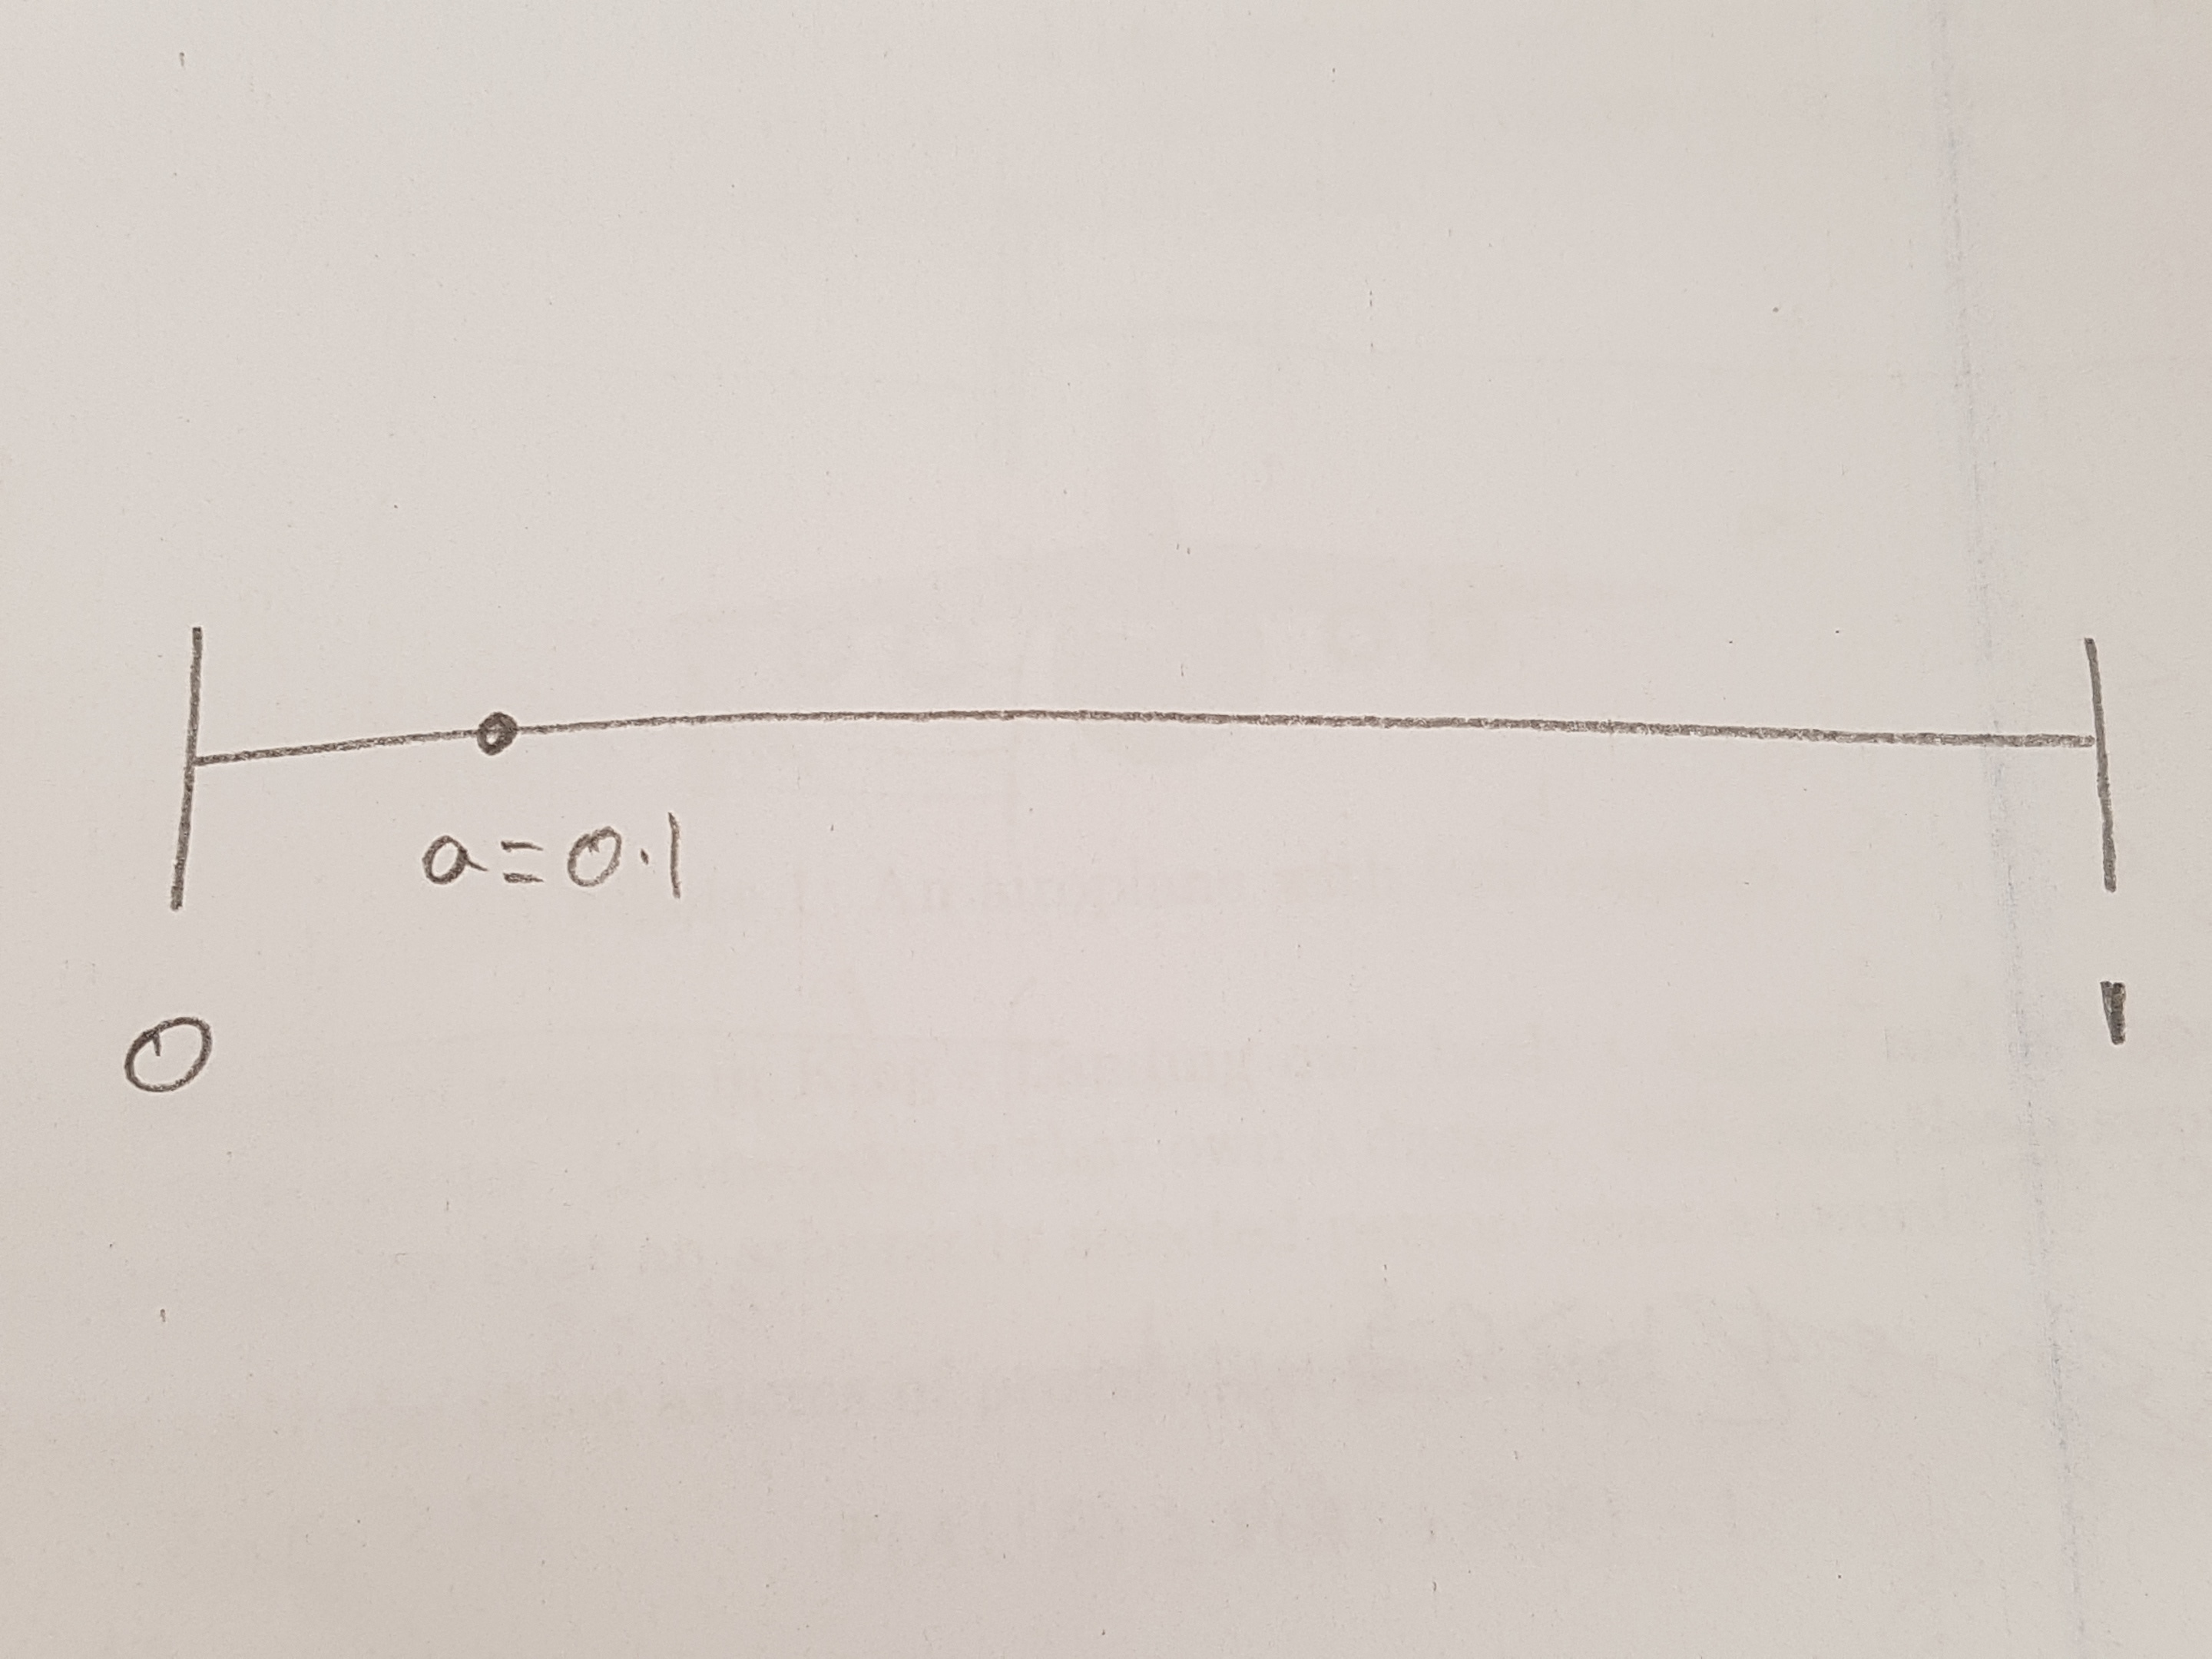
\includegraphics[width=5in]{a.jpg}
\end{figure}

Now we will add the second point. The second point can only be placed in the
shaded section since all sides must be less than 0.5.
\begin{figure}[H]
    \centering
    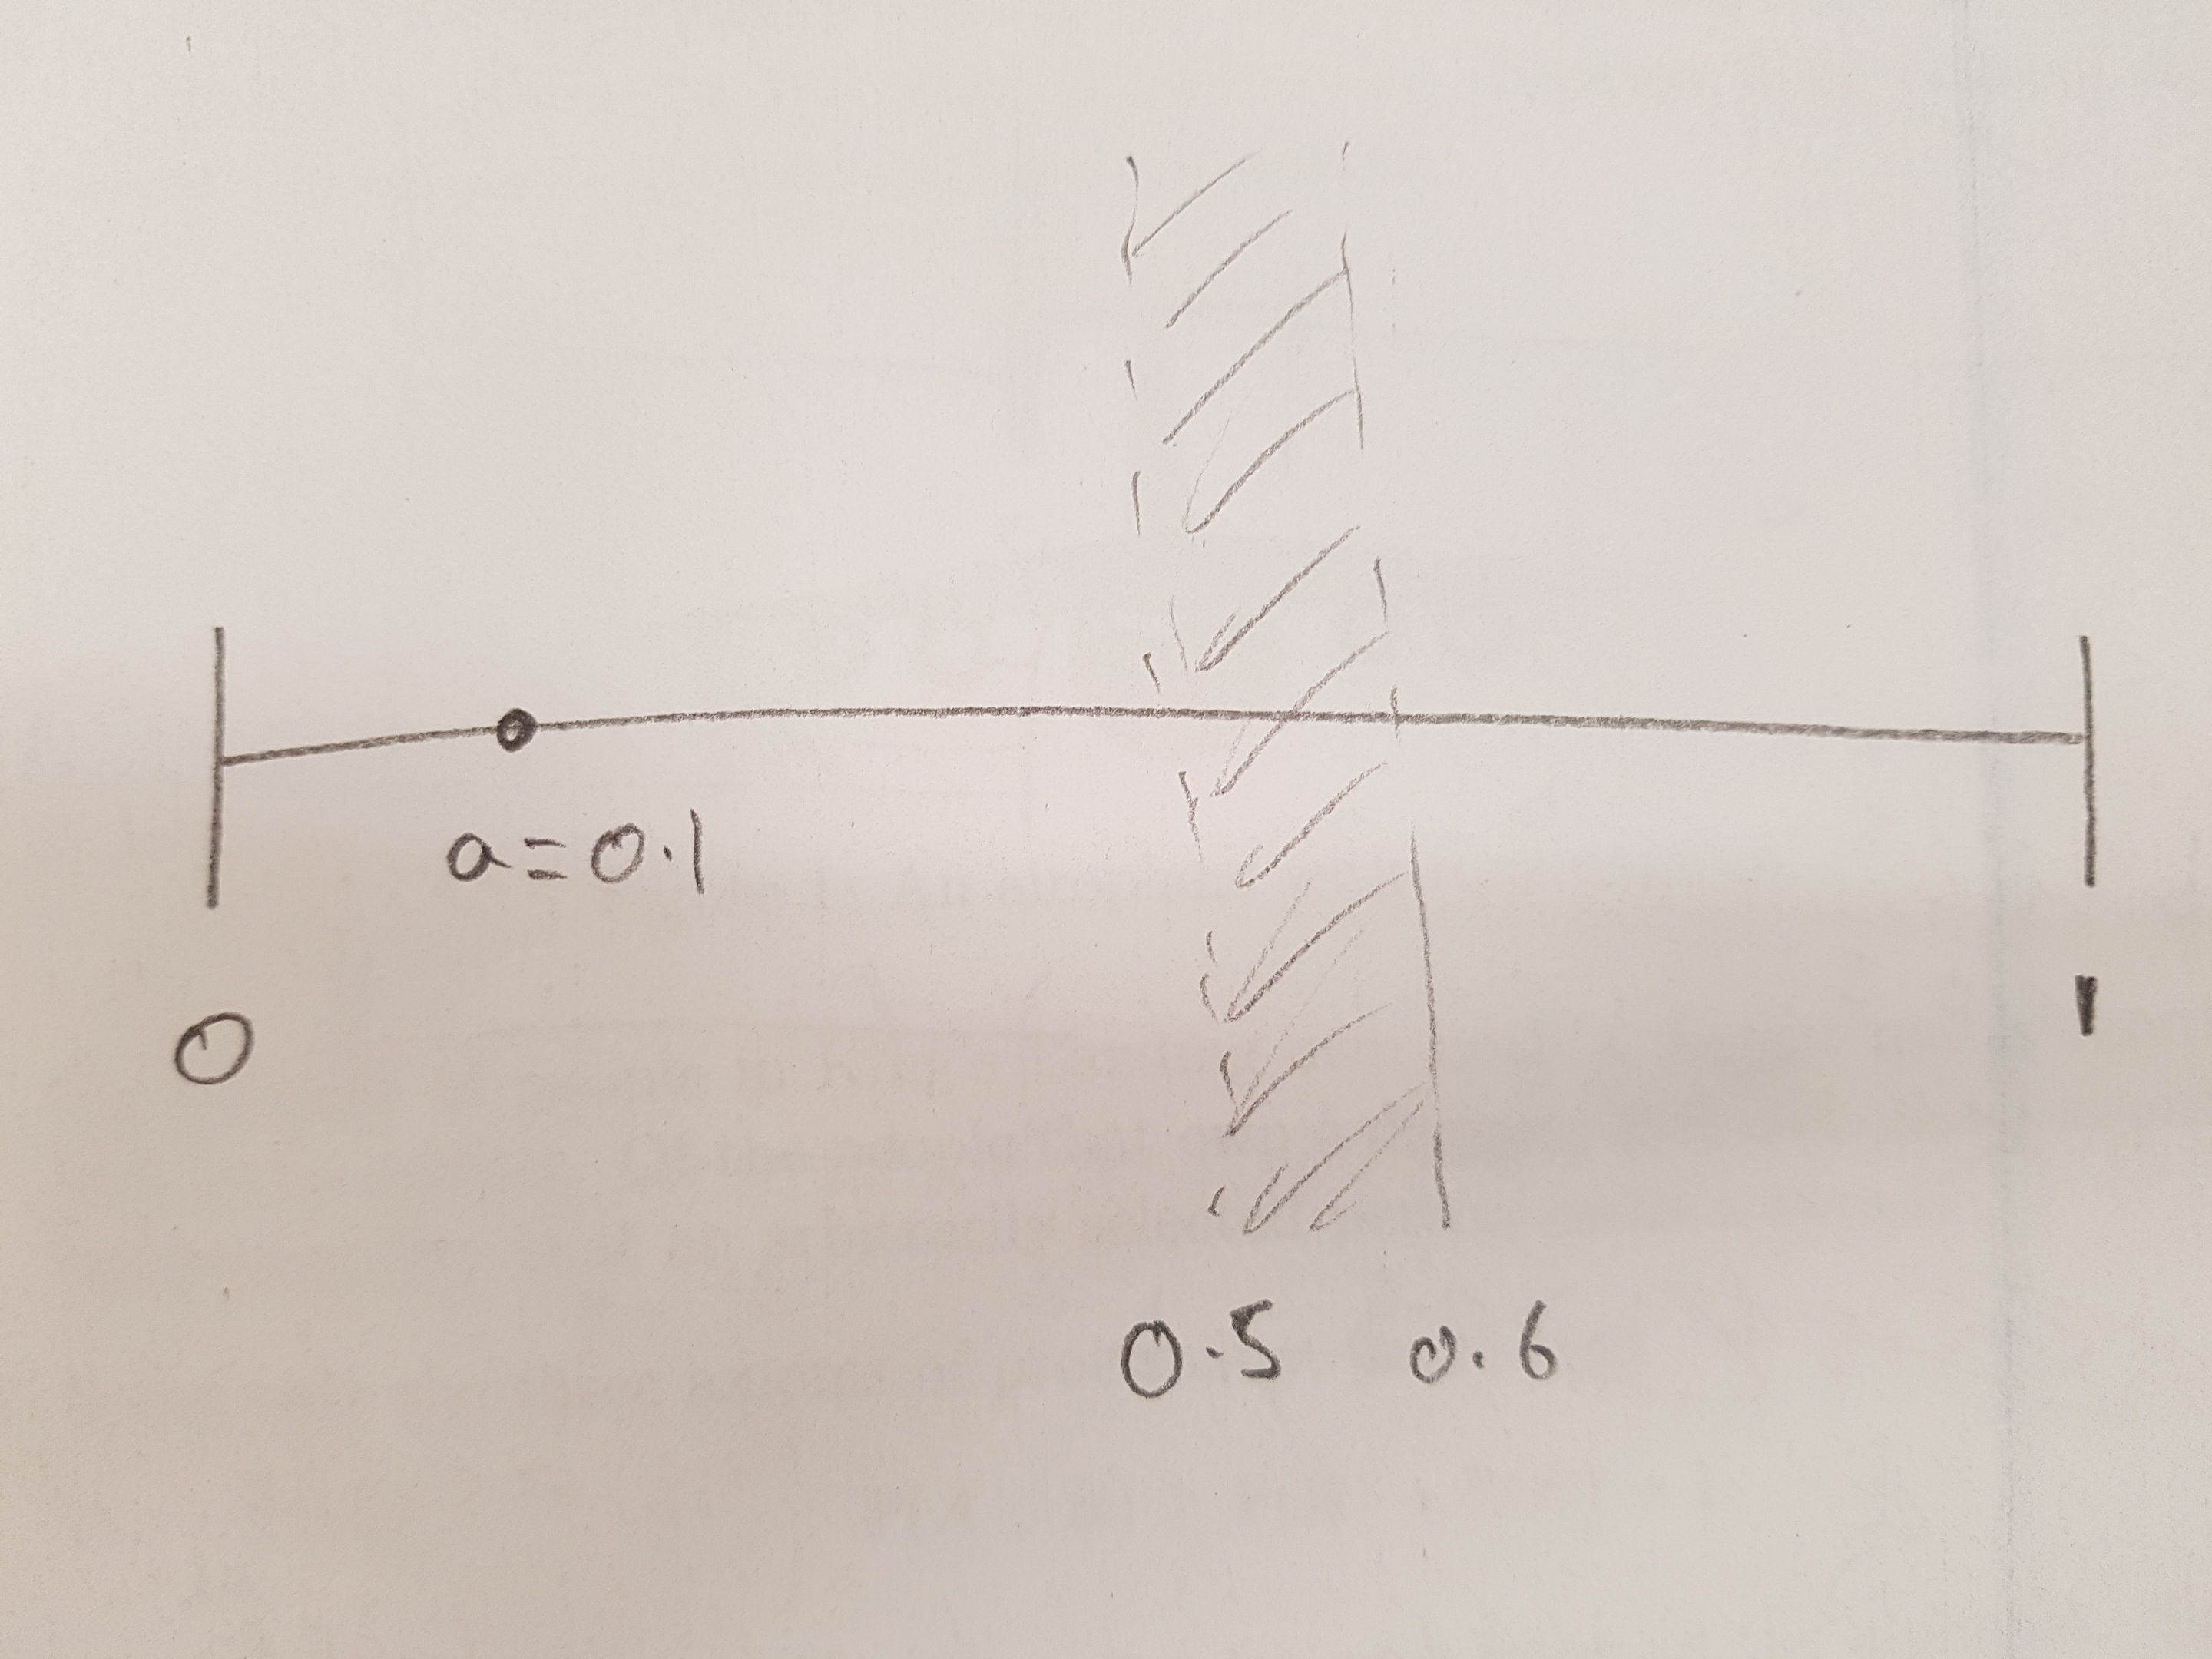
\includegraphics[width=5in]{b.jpg}
\end{figure}
The chance that the second point lands in this "sweet spot" section is 0.1 in
this example. But it can be generalised to whatever value of $a$ is.

With this we can generate a score function.
\begin{align*}
    x(a) &= 
    \begin{cases}
        a & a < 0.5 \\
        1 - a & a > 0.5 \\
    \end{cases}
\end{align*}

This function gives the probability of "success" at each possible value of $a$.
Now we use this scoring with the uniform distribution of $a$, $f(a) = 1$
to find the expected probability. 
\begin{align*}
    \int_a x(a) f(a) da &= \int_a x(a) da \\
    &= \int_0^{0.5} x(a) da + \int_{0.5}^1 x(a) da \\
    &= \left. 0.5 a^2 \right|_0^{0.5} + \left. a - 0.5 a^2 \right|_{0.5}^1 \\
    &= 0.125 + 0.125 \\
    &= 0.25 \\
\end{align*}

Thus the expected probability is 0.25.
\end{document}
